
\documentclass[12pt,a4paper]{article}
% ==========================================
% GRAFICI E TABELLE CAPITOLO 3
% ==========================================
% Nota: Aggiungere nel preambolo:

\usepackage{pgfplots}
\usepackage{tikz}
\usepackage{booktabs}
\usepackage{array}
\usepackage{multirow}
\usepackage{caption}
\usepackage{amsmath}    
\usepackage{amssymb}
\usepgfplotslibrary{fillbetween}

\usepackage{pgfplotstable}
\usepackage{graphicx}
\usepackage{hyperref}
\usepackage{geometry}
\geometry{a4paper, margin=1in}

\pgfplotsset{compat=1.18}
\begin{document}



% ==========================================
% TABELLA 3.1: Analisi Costo-Beneficio Ridondanza Alimentazione
% ==========================================

\begin{table}[htbp]
\centering
\caption{Analisi Costo-Beneficio Ridondanza Alimentazione per Classe Dimensionale}
\label{tab:ridondanza-alimentazione}
\begin{tabular}{@{}lcccccc@{}}
\toprule
\textbf{Classe} & \textbf{Config.} & \textbf{MTBF} & \textbf{Downtime} & \textbf{Costo} & \textbf{ROI} & \textbf{Raccom.} \\
\textbf{Dimensionale} & & \textbf{(ore)} & \textbf{(ore/anno)} & \textbf{(€/m²)} & \textbf{(mesi)} & \\
\midrule
<500 m² & N+0 & 8.760 & 8,76 & 45 & -- & No \\
        & N+1 & 52.560 & 1,46 & 78 & 18 & \checkmark \\
        & N+2 & 262.800 & 0,29 & 125 & 36 & -- \\
\midrule
500-1000 m² & N+0 & 8.760 & 8,76 & 52 & -- & No \\
            & N+1 & 52.560 & 1,46 & 89 & 14 & \checkmark \\
            & N+2 & 262.800 & 0,29 & 142 & 28 & Opz. \\
\midrule
>1000 m² & N+0 & 8.760 & 8,76 & 58 & -- & No \\
         & N+1 & 52.560 & 1,46 & 98 & 16 & Min. \\
         & N+2 & 262.800 & 0,29 & 156 & 22 & \checkmark \\
\bottomrule
\end{tabular}
\end{table}

% ==========================================
% FIGURA 3.1: Correlazione Investimenti-Availability
% ==========================================

\begin{figure}[htbp]
\centering
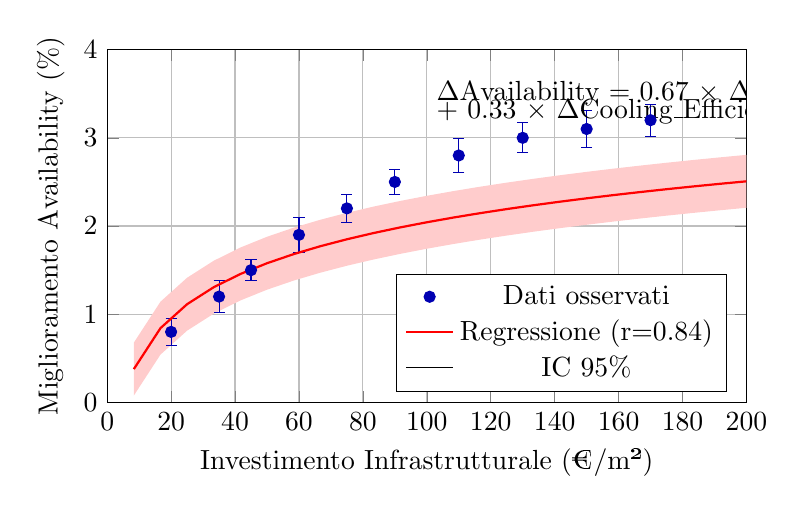
\begin{tikzpicture}
\begin{axis}[
    width=0.8\textwidth,
    height=0.5\textwidth,
    xlabel={Investimento Infrastrutturale (€/m²)},
    ylabel={Miglioramento Availability (\%)},
    xmin=0, xmax=200,
    ymin=0, ymax=4,
    grid=major,
    legend pos=south east,
    ]
    
    % Dati scatter plot
    \addplot[
        only marks,
        mark=*,
        mark size=2pt,
        color=blue!70!black,
        error bars/.cd,
        y dir=both,
        y explicit,
    ] coordinates {
        (20,0.8) +- (0,0.15)
        (35,1.2) +- (0,0.18)
        (45,1.5) +- (0,0.12)
        (60,1.9) +- (0,0.20)
        (75,2.2) +- (0,0.16)
        (90,2.5) +- (0,0.14)
        (110,2.8) +- (0,0.19)
        (130,3.0) +- (0,0.17)
        (150,3.1) +- (0,0.21)
        (170,3.2) +- (0,0.18)
    };
    
    % Linea di regressione
    \addplot[
        thick,
        color=red,
        domain=0:200,
    ] {0.67*ln(x/10) + 0.5};
    
    % Confidence interval
    \addplot[
        name path=upper,
        draw=none,
        domain=0:200,
    ] {0.67*ln(x/10) + 0.5 + 0.3};
    
    \addplot[
        name path=lower,
        draw=none,
        domain=0:200,
    ] {0.67*ln(x/10) + 0.5 - 0.3};
    
    \addplot[red!20] fill between[of=upper and lower];
    
    \legend{Dati osservati, Regressione (r=0.84), IC 95\%}
    
    % Annotazione
    \node[anchor=west] at (axis cs:100,3.5) {$\Delta$Availability = 0.67 $\times$ $\Delta$Power\_Reliability};
    \node[anchor=west] at (axis cs:100,3.3) {+ 0.33 $\times$ $\Delta$Cooling\_Efficiency};
    
\end{axis}
\end{tikzpicture}
\caption{Correlazione tra Investimenti Infrastrutturali e Miglioramento Availability}
\label{fig:correlazione-investimenti}
\end{figure}

% ==========================================
% FIGURA 3.2: Decomposizione Riduzione ASSA
% ==========================================

\begin{figure}[htbp]
\centering
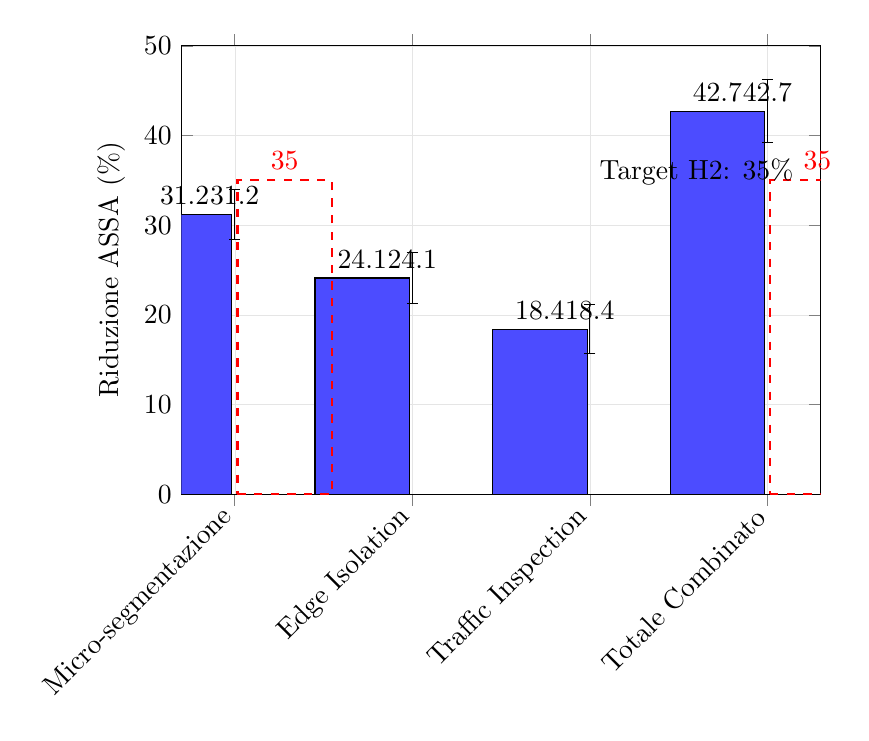
\begin{tikzpicture}
\begin{axis}[
    ybar,
    bar width=1.2cm,
    width=0.8\textwidth,
    height=0.6\textwidth,
    ylabel={Riduzione ASSA (\%)},
    symbolic x coords={Micro-segmentazione,Edge Isolation,Traffic Inspection,Totale Combinato},
    xtick=data,
    x tick label style={rotate=45,anchor=east},
    ymin=0, ymax=50,
    nodes near coords,
    nodes near coords align={vertical},
    grid=major,
    grid style={line width=.1pt, draw=gray!20},
    ]
    
    \addplot[fill=blue!70] coordinates {
        (Micro-segmentazione,31.2)
        (Edge Isolation,24.1)
        (Traffic Inspection,18.4)
        (Totale Combinato,42.7)
    };
    
    % Error bars
    \addplot[
        only marks,
        error bars/.cd,
        y dir=both,
        y explicit,
    ] coordinates {
        (Micro-segmentazione,31.2) +- (0,2.8)
        (Edge Isolation,24.1) +- (0,2.8)
        (Traffic Inspection,18.4) +- (0,2.7)
        (Totale Combinato,42.7) +- (0,3.5)
    };
    
    % Linea target H2
    \addplot[
    thick,
    dashed,
    color=red,
] coordinates {(Micro-segmentazione,35) (Totale Combinato,35)};
    
    \node[anchor=west] at (axis cs:Traffic Inspection,36) {Target H2: 35\%};
    
\end{axis}
\end{tikzpicture}
\caption{Decomposizione della Riduzione ASSA per Componente Architetturale}
\label{fig:riduzione-assa}
\end{figure}

% ==========================================
% TABELLA 3.2: Analisi TCO Strategie Migrazione
% ==========================================

\begin{table}[htbp]
\centering
\caption{Analisi Comparativa TCO per Strategia di Migrazione - 5 Year NPV}
\label{tab:tco-migrazione}
\begin{tabular}{@{}lcccccc@{}}
\toprule
\textbf{Strategia} & \textbf{CAPEX} & \textbf{OPEX} & \textbf{Time to} & \textbf{ROI} & \textbf{NPV 5Y} & \textbf{Risk} \\
 & \textbf{(€K/app)} & \textbf{Reduction} & \textbf{Migration} & \textbf{Break-even} & \textbf{(€K)} & \textbf{Score} \\
\midrule
\multirow{2}{*}{Lift-and-Shift} & 8.2 & 23.4\% & 3.2 mesi & 14.3 mesi & 47.3 & Low \\
 & (±1.2) & (±4.1\%) & (±0.8) & (±2.1) & (±8.2) & (2/10) \\
\midrule
\multirow{2}{*}{Replatforming} & 24.7 & 41.3\% & 7.8 mesi & 19.7 mesi & 89.4 & Medium \\
 & (±3.8) & (±5.3\%) & (±1.2) & (±3.2) & (±12.7) & (5/10) \\
\midrule
\multirow{2}{*}{Refactoring} & 87.3 & 58.9\% & 16.4 mesi & 28.1 mesi & 156.8 & High \\
 & (±12.4) & (±6.7\%) & (±2.3) & (±4.6) & (±23.4) & (7/10) \\
\bottomrule
\end{tabular}
\end{table}

% ==========================================
% FIGURA 3.3: Evoluzione TCO e Availability
% ==========================================

\begin{figure}[htbp]
\centering
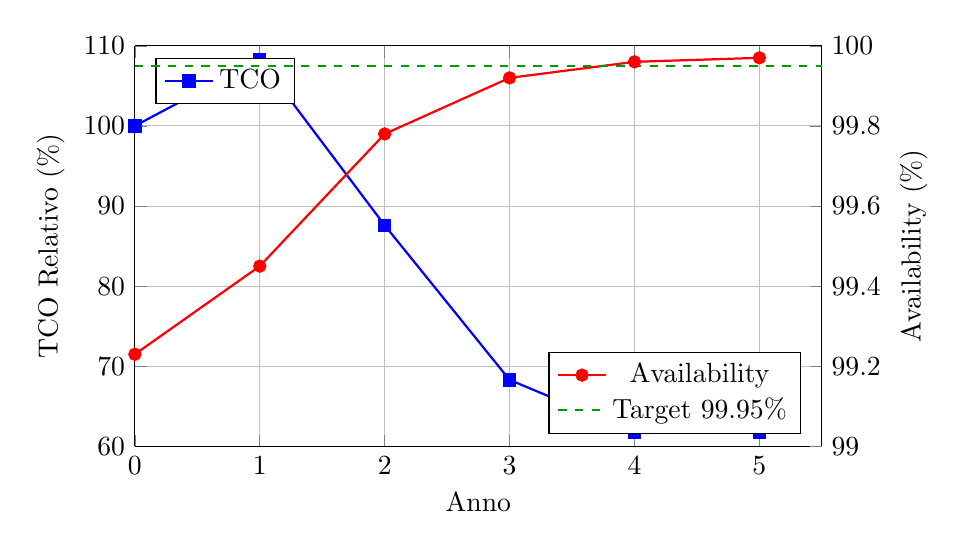
\begin{tikzpicture}
\begin{axis}[
    width=0.85\textwidth,
    height=0.55\textwidth,
    axis y line*=left,
    xlabel={Anno},
    ylabel={TCO Relativo (\%)},
    xmin=0, xmax=5.5,
    ymin=60, ymax=110,
    xtick={0,1,2,3,4,5},
    grid=major,
    legend pos=north west,
    ]
    
    % TCO line
    \addplot[
        thick,
        mark=square*,
        color=blue,
    ] coordinates {
        (0,100)
        (1,108.3)
        (2,87.6)
        (3,68.3)
        (4,61.8)
        (5,61.8)
    };
    \addlegendentry{TCO}
    
\end{axis}

% Second y-axis for Availability
\begin{axis}[
    width=0.85\textwidth,
    height=0.55\textwidth,
    axis y line*=right,
    axis x line=none,
    ylabel={Availability (\%)},
    xmin=0, xmax=5.5,
    ymin=99.0, ymax=100,
    ytick={99.0,99.2,99.4,99.6,99.8,100.0},
    legend pos=south east,
    ]
    
    % Availability line
    \addplot[
        thick,
        mark=*,
        color=red,
    ] coordinates {
        (0,99.23)
        (1,99.45)
        (2,99.78)
        (3,99.92)
        (4,99.96)
        (5,99.97)
    };
    \addlegendentry{Availability}
    
    % Target line
    \addplot[
        thick,
        dashed,
        color=green!60!black,
        domain=0:5.5,
    ] {99.95};
    \addlegendentry{Target 99.95\%}
    
\end{axis}
\end{tikzpicture}
\caption{Evoluzione TCO e Availability durante Migrazione Cloud}
\label{fig:evoluzione-tco}
\end{figure}

% ==========================================
% FIGURA 3.4: Distribuzione Rischio Monte Carlo
% ==========================================

\begin{figure}[htbp]
\centering
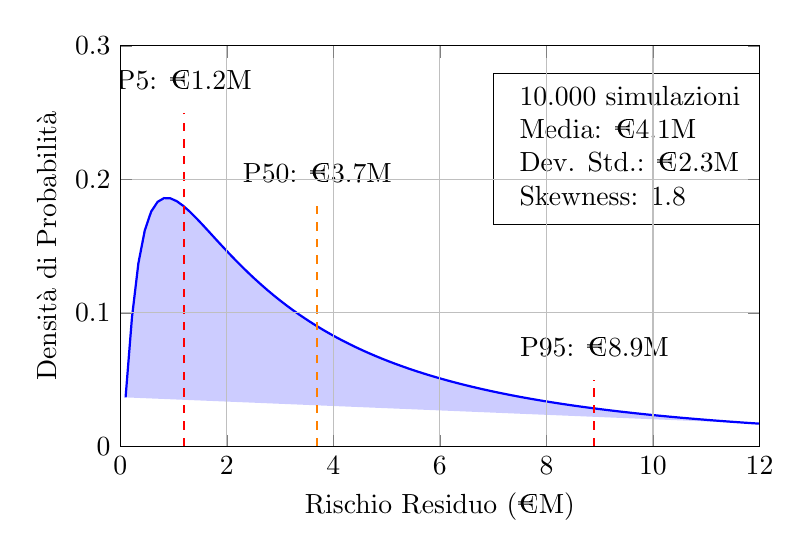
\begin{tikzpicture}
\begin{axis}[
    width=0.8\textwidth,
    height=0.55\textwidth,
    xlabel={Rischio Residuo (€M)},
    ylabel={Densità di Probabilità},
    xmin=0, xmax=12,
    ymin=0, ymax=0.3,
    grid=major,
    area style,
    ]
    
    % Distribuzione log-normale
    \addplot[
        thick,
        color=blue,
        fill=blue!20,
        domain=0.1:12,
        samples=100,
    ] {1/(x*1.2*sqrt(2*pi))*exp(-(ln(x)-1.3)^2/(2*1.2^2))};
    
    % Percentili verticali
    \draw[thick,dashed,red] (1.2,0) -- (1.2,0.25);
    \draw[thick,dashed,orange] (3.7,0) -- (3.7,0.18);
    \draw[thick,dashed,red] (8.9,0) -- (8.9,0.05);
    
    % Labels
    \node[anchor=south] at (axis cs:1.2,0.26) {P5: €1.2M};
    \node[anchor=south] at (axis cs:3.7,0.19) {P50: €3.7M};
    \node[anchor=south] at (axis cs:8.9,0.06) {P95: €8.9M};
    
    % Legenda manuale
    \node[anchor=north west,draw,fill=white] at (axis cs:7,0.28) {
        \begin{tabular}{l}
        10.000 simulazioni\\
        Media: €4.1M\\
        Dev. Std.: €2.3M\\
        Skewness: 1.8
        \end{tabular}
    };
    
\end{axis}
\end{tikzpicture}
\caption{Distribuzione del Rischio - Simulazione Monte Carlo}
\label{fig:monte-carlo}
\end{figure}

\end{document}